\subsection*{A0}
Le département ASI a développé un système, qu'on appellera FAKE, basé sur deux applications communiquant via un broker JMS. Ces 2 applications ainsi que le broker JMS sont déployées sur 3 machines différentes. L'objectif est d'utiliser les techniques de \textit{containerization of software}, pilotés par des outils d'intégration et de livraison continue, pour faciliter le test et la mise en production du système FAKE.

\subsection*{A1}
    \subsubsection*{Questions d'amorces}
    Le terme de \textit{containerization of software} désigne le fait de réaliser un conteneur pour une application spécifique où l'on inclut les éléments suivants : un système d'exploitation, des paquets de dépendances et l'application en elle-même. Au lieu d'avoir un binaire (ou équivalent) d'une application, qui doit ensuite être déployé dans un environnement répondant aux besoins de l'application, on réalise un package englobant les dépendances de l'application. Puisque l'on dispose de conteneurs de l'application, on peut alors en théorie déployer plus facilement celle-ci sur de multiples machines, ce qui permet d'assurer la scalabilité d'un système. Ceci est la tendance de l'utilisation de \textit{commodity hardware} qui consiste à multiplier l'utilisation de serveurs peu puissants plutôt que d'investir dans un serveur extrêmement puissant et coûteux.\\

    La différence entre la virtualisation et les conteneurs n'est pas toujours facile à comprendre. De manière générale, la virtualisation apporte une isolation importante mais à un coût plus fort comme chaque machine virtuelle fait tourner son propre noyau et système d'exploitation. Les conteneurs offrent moins d'isolation mais sont beaucoup moins gourmands en ressources car ils partagent certaines parties du noyau et du système d'exploitation du serveur sur lequel ils tournent. Ceci est illustré dans la figure~\ref{fig:vms-containers}.\\

    \begin{figure}[h]
      \centering
      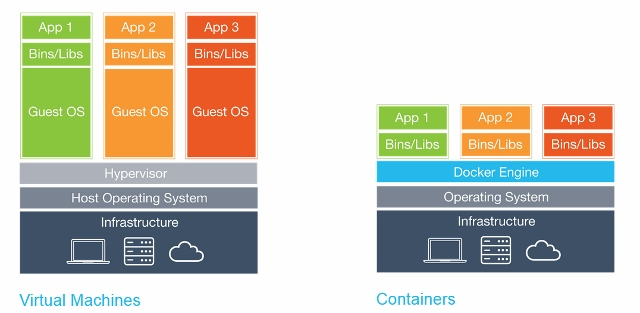
\includegraphics[width=0.8\textwidth]{images/vms-containers.jpg}
      \caption{Différences entre machine virtuelles et conteneurs. Crédit : \url{http://fossbytes.com/getting-started-with-docker-intro-to-containers-world-part-1/}}
      \label{fig:vms-containers}
    \end{figure}

    Les conteneurs sont souvent utilisés pour effectuer de l'intégration continue (lancer des tests lorsqu'un programme est modifié) ou dans le cadre d'une chaîne de livraison continue (passage d'un environnement de test à du staging puis de la production). En effet les conteneurs facilitent le déploiement car l'application est packagée avec ses dépendances et peut tourner sur plusieurs systèmes d'exploitation ou types de machines physiques.\\

    Les conteneurs sont souvent aussi utilisés pour gérer les microservices. Les microservices sont de petits composants indépendants d'une architecture (API d'authentification, de recherche de commandes, de gestion des favoris\dots) qui peuvent avoir le besoin de changer de taille rapidement en fonction de leurs usages et de la demande. Les conteneurs permettent de répondre à ces besoins.

    \subsubsection*{Liste de mots clés}
        \begin{itemize}
            \item Intégration continue
            \item Virtualisation
            \item Conteneurisation
            \item Tests
            \item Scalabilité
            \item Déploiement
            \item Microservice
            \item Livraison continue
            \item Conteneurs logiciels
            \item Portabilité d'applications
        \end{itemize}

\subsection*{A2}
    \begin{itemize}
        \item \textit{How Clay.Io Built Their 10x Architecture Using AWS, Docker, HAProxy, And Lots More} \url{http://highscalability.com/blog/2014/10/6/how-clayio-built-their-10x-architecture-using-aws-docker-hap.html} -- mise en place d'une architecture dans le cloud à l'aide de conteneurs, scalable, permettant de s'adapter à la demande
        \item \textit{Building a Continuous Integration Pipeline with Docker} \url{https://www.docker.com/sites/default/files/UseCase/RA_CI%20with%20Docker_08.25.2015.pdf} -- facilite l'intégration continue à l'aide de conteneurs préconfigurés
        \item \textit{Faster Builds with Container-Based Infrastructure and Docker} \url{http://blog.travis-ci.com/2014-12-17-faster-builds-with-container-based-infrastructure/} -- passage d'une infrastructure se basant sur de la virtualisation à des conteneurs
    \end{itemize}

\subsection*{A3}
    \begin{itemize}
        \item Deploy web apps with Docker \url{https://leanpub.com/deploy-web-apps-with-docker} Chapitre 1 : \enquote{What is Docker and why should you use it?}
        \item The Docker Book: Containerization is the new virtualization \url{http://www.amazon.fr/gp/product/B00LRROTI4} Chapitre 2 : \enquote{What can you use Docker for?}
        \item Docker: Up and Running \url{http://www.amazon.fr/Docker-Up-Running-Karl-Matthias-ebook/dp/B00ZGRS4XM/} Chapitre 9 : \enquote{Deploying containers at scale in public and private clouds}
    \end{itemize}

\subsection*{A4}
    \subsubsection*{Travis CI}
    Travis CI est une plateforme d'intégration continue qui permet de packager et de tester des logiciels qui sont hébergés sur GitHub. Travis CI détecte dès qu'un commit a été push sur GitHub et lancera alors une suite de commandes, paramétrables grâce à un fichier de configuration écrit en YAML nommé \texttt{.travis.yml}.\\

    Travis CI s'appuie sur l'infrastructure d'Amazon Web Services et utilise des conteneurs Docker pour exécuter les tests. Travis CI Pro offre les mêmes fonctionnalités que la version gratuite de Travis CI, mais pour les répertoires privés hébergés sur GitHub.

    \subsubsection*{Docker}
    Docker est un logiciel libre qui automatise le déploiement d'applications dans des conteneurs logiciels. Selon la firme de recherche sur l'industrie 451 Research, « Docker est un outil qui peut empaqueter une application et ses dépendances dans un conteneur virtuel, qui pourra être exécuté sur n'importe quel serveur Linux ».\\

    La technologie de conteneur de Docker peut être utilisée pour étendre des systèmes distribués de façon à ce qu'ils s'exécutent de manière autonome depuis une seule machine physique ou une seule instance par nœud. Cela permet aux nœuds d'être déployés au fur et à mesure que les ressources sont disponibles, offrant un déploiement transparent et similaire aux PaaS pour des systèmes comme Apache Cassandra, Riak ou d'autres systèmes distribués.

    \subsubsection*{Kubernetes}
    Google est derrière Kubernetes, un gestionnaire open source de conteneurs. Ce dernier permet de déployer des conteneurs sur un lot de machines, d’en surveiller le bon fonctionnement et d’assurer leur réplication. Une offre idéale pour administrer des conteneurs Linux sur une infrastructure de type cloud public. Microsoft s'est assuré que Kubernetes fonctionne bien sur Azure, Red Hat a fait de même. Docker et CoreOS assurent également la compatibilité avec Kubernetes et se sont engagés à assurer la compatibilité dans le futur, avec l'aide entre autre d'IBM.

\subsection*{A5}
    \begin{itemize}
        \item \textbf{Adaptability}: characterizes the ability of the system to change to new specifications or operating environments.
        \item \textbf{Installability}: characterizes the effort required to install the software.
        \item \textbf{Fault tolerance}: characterizes the ability of software to withstand (and recover) from component, or environmental, failure.
    \end{itemize}

\subsection*{A6}
    \begin{itemize}
        \item Adaptability
            \begin{itemize}
                \item Number of functions
                \item Number of datastructures
                \item Operation time / number of functions
            \end{itemize}
        \item Installability
            \begin{itemize}
                \item Number of installation steps
                \item Number of setup operations
                \item Number of step / number of setup operations = number of steps by setup operation
            \end{itemize}
        \item Fault tolerance
            \begin{itemize}
                \item Number of failures
                \item Number of test cases
                \item Number of failure + Number of breakdowns x 10
            \end{itemize}
    \end{itemize}

\subsection*{A7}
